\doublespacing

Looking at the plot of the difference between the two-body effective potential and the bare Coulomb potential ($V_{eff}-V_{Coul}$) in real space as a function of the chord distance $r$ between electrons on the Haldane sphere in Fig. \ref{fig:exc_disp_kappas}, we see that the magnitude of the difference at any distance for magnetic monopole strength $Q=7.5$ increases with increasing Landau level mixing (LLM) parameter $\kappa$. We also notice that the differences for every $\kappa$ value intersect at $V_{eff}-V_{Coul}=0$, or $V_{eff}=V_{Coul}$, for $r\approx0.8$. In this Appendix, we want to explain the cause of this and understand how this difference changes as a function of $Q$. 

From the modified Park potential (Eq. \ref{modPark}), we have
\begin{equation}\label{potDiff}
  V_{eff}-V_{Coul}=b_1e^{-\beta_1r}+b_2r^2e^{-\beta_2r}. 
\end{equation}
We can solve for the distance at which the effective potential intersects the Coulomb potential, $r(V_{eff}=V_{Coul})$, by setting the left side of the equation above to 0 and solving for $r$. This expression depends linearly on $b_i$ which depend linearly on $\kappa$, and on $\beta_i$ which do not depend on $\kappa$, so the $\kappa$ dependence of $r(V_{eff}=V_{Coul})$ is cancelled out. We used the Python library SymPy so solve for the unique solutions of $r(V_{eff}=V_{Coul})$ \cite{sympy}, 
\begin{equation}\label{r_v_eff_eq_v_coul}
\left[\frac{2 W\left(\frac{\sqrt{-\frac{b_{1}}{b_{2}}}\left(-\beta_{1}+\beta_{2}\right)}{2}\right)}{\beta_{1}-\beta_{2}}, \frac{2 W\left(\frac{\sqrt{-\frac{b_{1}}{b_{2}}}\left(\beta_{1}-\beta_{2}\right)}{2}\right)}{\beta_{1}-\beta_{2}}\right],
\end{equation}
where $W$ is the Lambert W function. We can use the following sample parameter values to determine which expression to use: $b_1(7.5, 2.2)=-6.879503$, $b_2(7.5, 2.2)=1.105104$, $\beta_1(7.5)=4.485793$ and $\beta_2(7.5)=1.468513$. Since $\beta_1>\beta_2$, we have 
\begin{equation}\label{r_v_eff_eq_v_coul_singl}
r(V_{eff}=V_{Coul})=\frac{2}{\beta_1-\beta_2}W\left(\frac{\beta_1-\beta_2}{2}\sqrt{\frac{-b_1}{b_2}}\right).
\end{equation}
We can plug in the sample parameter values to find $r(V_{eff}=V_{Coul},7.5)=0.774999$. The full expression of the distance where the effective potential intersects the Coulomb potential in real space as a function of $Q$ is as follows:
\begin{equation}
    \resizebox{\textwidth}{!}
     {
        r(V_{eff}=V_{Coul},Q)=\frac{2 W\left(\sqrt { \frac { Q ^ { 0 . 4 5 2 2 1 6} + 0 . 2 4 1 2 4 6} { 1 . 8 4 7 2 3 7 \cdot 1 0 ^ { - 5 } Q ^ { 2. 2 7 4 2 2 6} + 0 . 0 4 8 4 2 6} } \left(0.153363 Q^{0.537208}-0.005767 Q^{1.150906}+0.116654\right)\right)}{0.906035 Q^{0.537207}-0.034071 Q^{1.151906}+0.689167}.
     }
\end{equation}

We can view the behavior of $r(V_{eff}=V_{Coul},Q)$ in the plot in Fig. \ref{fig:r_vEff_eq_vCoul_vs_q}. It starts to diverge near $Q\approx253.5$, which corresponds to $N=169$ electrons at filling factor $\nu=1/3$ in the lowest Landau level (LLL). It appears that for $Q\geq253.5$, $V_{eff}$ starts below $V_{Coul}$, then quickly converges to it from below without ever rising above (for $Q=252.0$, $V_{eff}$ is within 1\% of $V_{Coul}$ for all points $r\gtrsim0.345$). We confirm this behavior of the difference with respect to $Q$ in the plot in Fig. \ref{fig:vEff_minus_vCoul_vs_r_qs}.

\begin{figure}[H]
\begin{center}
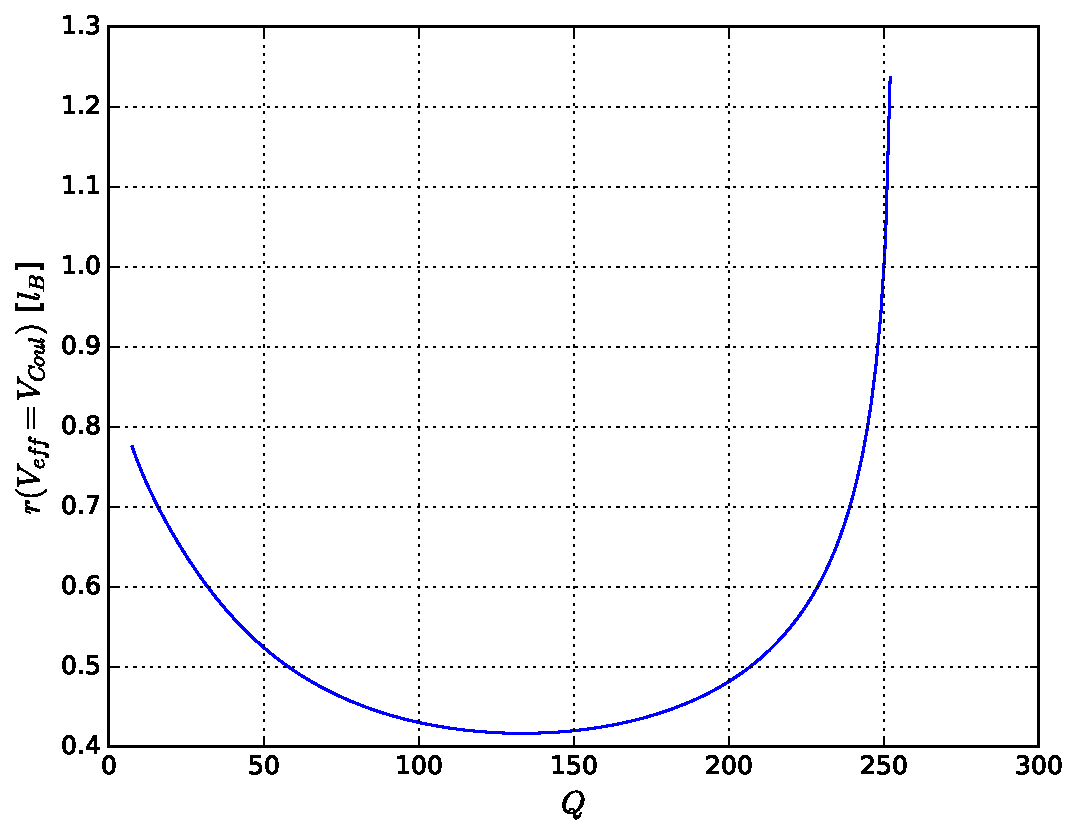
\includegraphics[width=10cm, angle=0]{ThesisCSULBLatexTemplate/figures/r_vEff_eq_vCoul_vs_q.pdf}
\caption[The chord distance between electrons on the Haldane sphere where the effective potential intersects the bare Coulomb potential in real space for all LLM parameter values.]{The chord distance between electrons on the Haldane sphere where the effective potential intersects the bare Coulomb potential in real space for all LLM parameter values. We plot $r(V_{eff}=V_{Coul})$ as a function of the magnetic monopole strength $Q$ from data collected in the LLL with filling factor $\nu=1/3$. It diverges near $Q\approx253.5$.}
\label{fig:r_vEff_eq_vCoul_vs_q} 
\end{center}
\end{figure}

\begin{figure}[p]
\begin{center}
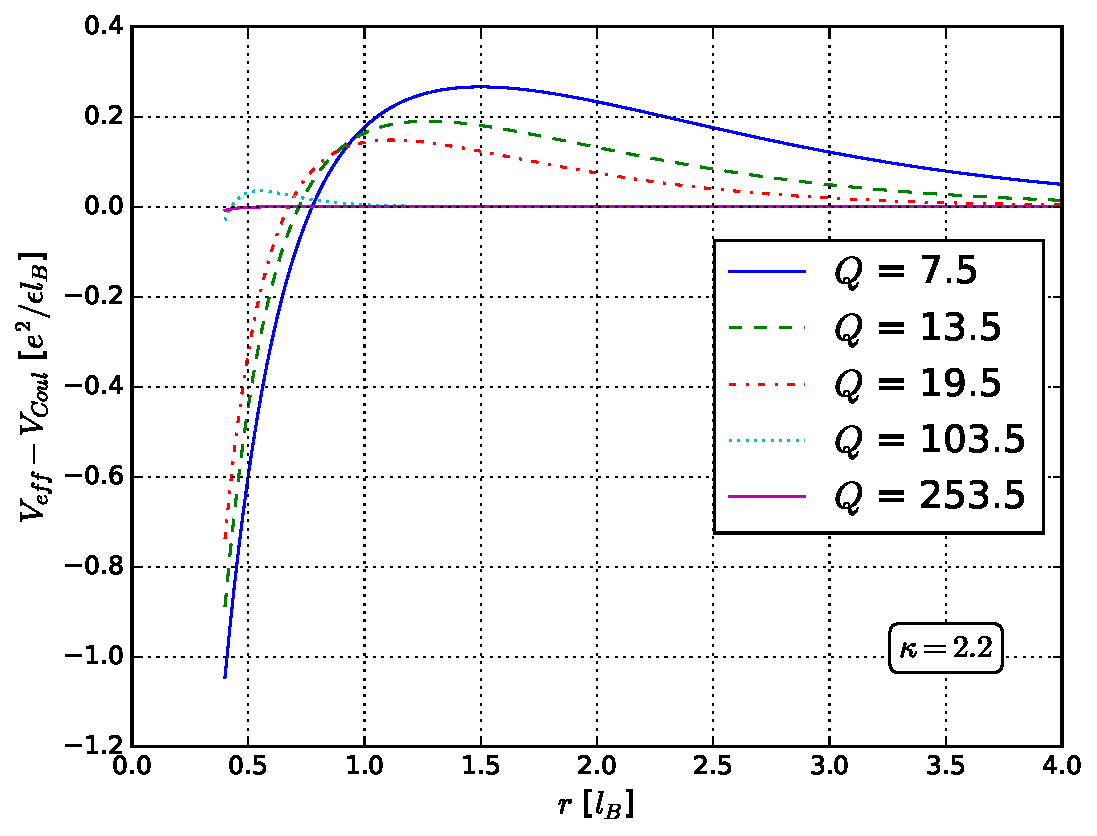
\includegraphics[width=10cm, angle=0]{ThesisCSULBLatexTemplate/figures/vEff_minus_vCoul_vs_r_qs.pdf}
\caption[The difference between the effective potential and bare Coulomb potential in real space at different magnetic monopole strengths.]{The difference between the effective potential and bare Coulomb potential in real space at different magnetic monopole strengths.We plot $V_{eff}-V_{Coul}$ as a function of the chord distance between electrons on the Haldane sphere $r$ in the LLL at filling factor $\nu=1/3$, LLM parameter $\kappa=2.2$, and $Q\in\{7.5,13.5,19.5,103.5,253.5\}$. For smaller values of $Q$, the difference is negative at small distances, then positive at larger differences before converging to zero at far distances. When $Q\gtrsim253.5$, the difference quickly converges to 0 from below without ever reaching positive values.}
\label{fig:vEff_minus_vCoul_vs_r_qs} 
\end{center}
\end{figure}

\singlespacing